\chapter{Эксплутационные процессы ядерных реакторов}


\section{Ядерные энергетические установки}\label{Reactor}

\subsection{Устройство энергетического реактора}

Рассмотрим устройство энергетического реактора на примере ядерной энергетической установки БН-350.
Реактор БН-350 --- первый реактор на быстрых нейтронах энергетического  назначения (рис.~\ref{pic:basic-view}).
\begin{figure}[p]
\center{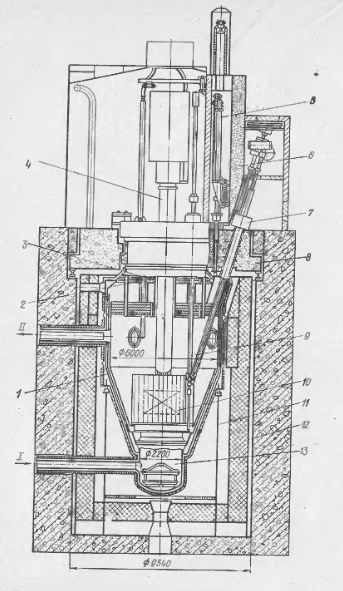
\includegraphics{basic-view}}
\caption[Общий вид реактора БН-350]{Общий вид реактора БН-350: 1 -- корпус реактора; 2 -- большая поворотная пробка; 3 -- малая поворотная пробка; 4 -- центральная поворотная колонка с механизмом СУЗ; 5 -- механизм передачи сборок; 6 -- передаточный бокс; 7 -- элеватор загрузки-выгрузки; 8 -- верхняя неподвижная защита; 9 -- механизм перегрузки; 10 -- активная зона; 11 -- опора реактора; 12 -- боковая защита; 13 -- напорная камера; I -- вход натрия; II -- выход натрия}
\label{pic:basic-view}
\end{figure}
В его конструкцию были заложены многие технические решения, выработанные на реакторе БОР-60, и впоследствии реализованные в конструкциях реакторов БН-600 и БН-800.
Внутри герметичного корпуса реактора, выполненного в виде бака переменного диаметра, расположены тепловыделяющие сборки (ТВС) активной зоны и боковой зоны воспроизводства, хранилище отработавших ТВС, отражатель нейтронов, механизмы системы перегрузки, стержни системы управления и защиты (СУЗ).
Натрий под давлением $~1$~МПа подводится от главных циркуляционных насосов (ГЦН) первого контура по шести напорным трубопроводам диаметром 500 мм в нижнюю часть корпуса реактора, образующую напорную камеру.
Сверху на камере закреплен напорный коллектор с установленными в нем ТВС.
В коллекторе поток теплоносителя распределяется по ТВС в соответствии с уровнем энерговыделения в них.
Он представляет собой прочную силовую конструкцию, воспринимающую весовую нагрузку от ТВС и других выемных частей реактора, а также внутренние давление теплоносителя.
Крепление коллектора к напорной камере допускает его извлечение и замену в случае необходимости.

Пройдя ТВС, нагретый натрий попадает в выходную смесительную камеру, откуда по шести сливным трубопроводам диаметром 600 мм отводится к промежуточным теплообменникам.

Активная зона набирается из шестигранных ТВС размером <<под ключ>> 96 мм. 
Каждая сборка содержит пучок гладкостержневых тепловыделяющих элементов (ТВЭЛов) диаметром 6,9 мм, расположенных с шагом 8 мм.
Топливо --- обогащенная двуокись урана.
Дистанцирование ТВЭЛов в пучке осуществляется проволокой, спирально навитой на оболочку ТВЭЛа.
Верхняя торцевая зона воспроизводства набирается из элементов увеличенного диаметра (12 мм) с двуокисью обедненного урана, установленных внутри сборки над пучком ТВЭЛов.
Гексагональная чехловая труба сборки несет давление теплоносителя, которое в нижней части значительно превышает давление в межкассетном пространстве реактора.
К чехлу сборки с обоих торцов приварены концевые детали цилиндрической формы: нижний хвостовик с боковыми отверстиями, через которые в ТВС поступает теплоноситель, и фигурная головка с выходными  окнами, предназначенная для захвата сборки механизмом перезагрузки.
Для уменьшения паразитных протечек натрия из напорного коллектора вдоль хвостовика сборки на нем предусмотрены лабиринтные уплотнения.
Зазор между ТВС принят минимальным (2 мм) исходя из условий нормального извлечения их при перезагрузке с учетом возможных при работе формоизменений.
Для пространственной фиксации сборок они дистанцируются с помощью выступов (<<платиков>>) в верхней части чехловых труб.

Часть гнезд в центральной области активной зоны занята органами СУЗ (рис.~\ref{pic:basic-grid})
\begin{figure}[ht]
\center{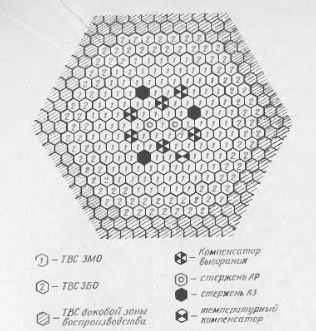
\includegraphics{basic-grid}}
\caption[Сетка СУЗ в реакторе БН-350]{Сетка СУЗ в реакторе БН-350: ЗМО -- зона малого обогащения, ЗБО -- зона большого обогащения}
\label{pic:basic-grid}
\end{figure}
Боковая зона воспроизводства общей толщиной 600 мм набрана из нескольких рядов ТВС, каждая из которых состоит из элементов диаметром 14,2 мм с двуокисью обедненного урана.
За внешним рядом сборок боковой зоны воспроизводства размещаются гнезда внутриреакторного хранилища, где отработавшие ТВС выдерживаются в течение интервала между перезагрузками реактора (2 месяца).
Необходимость выдержки сборок активной зоны перед выгрузкой из реактора обусловлена высоким уровнем остаточных тепловыделений в них.
В хранилище ТВС расхолаживаются теплоносителем, поступающим из напорного коллектора реактора.
После выдержки сборок значительно упрощается обращение с ними в тракте перегрузки.
Сборки боковой зоны воспроизводства имеют относительно низкое остаточное тепловыделение, поэтому предварительного охлаждения их перед выгрузкой не требуется.
Непосредственно за хранилищем устанавливается отражатель нейтронов из нескольких рядов стальных болванок с внешней конфигурацией ТВС (общая толщина 200 мм).

Натрий, заполняющий корпус реактора, образует свободный уровень, над которым находится аргоновая подушка.
Газовый объем служит для компенсации температурных расширений теплоносителя.
Вместе с тем он изолирует верхнюю часть реактора от горячего теплоносителя, выходящего из активной зоны, и защищает натрий от контакта с воздухом при случайной разгерметизации реактора.
Высота уровня над головками ТВС выбрана таким образом, чтобы транспортировка выгружаемых сборок проходила под слоем натрия, чем обеспечивается их надежное и эффективное охлаждение.
\cite{BH}


\subsection{Процесс перегрузки ядерного топлива}

Рассмотрим процесс перегрузки реактора БН-350.

Характерной особенностью конструкции реактора является то, что он не имеет съемной герметизирующей крышки, а перегрузка ТВС осуществляется без общего вскрытия корпуса герметичными дистанционно управляемыми механизмами под защитой инертного газа по закрытому тракту от реактора до внешнего хранилища.
Такое решение продиктовано специфическим требованием натриевой технологии --- недопустимостью контакта натрия с воздухом.
Сверху корпус реактора закрыт двумя многослойными плитами (<<пробками>>) верхней радиационной защиты.
Защитные пробки являются одновременно частью системы перегрузки реактора.
С их помощью осуществляются наведение внутриреакторного механизма перегрузки (ВМП) на ТВС, подлежащие перегрузке и перенос сборок внутри реактора. 
Эти операции выполняются совместным вращением обоих пробок --- большой, перекрывающей горловину реактора, и расположенной в ней эксцентрично малой пробки, в которую вмонтирован ВМП.
Обе пробки установлены на шаровых опорах, имеют по периферии зубчатый венец и электромеханические приводы, обеспечивающие их вращение по командам автоматизированной системы управления.
Поворотные пробки имеют значительный диаметр (большая пробка -- 4300 мм), поэтому создание надежного механического уплотнения по всему периметру, исключающего выход из реактора радиоактивного защитного газа, является весьма сложной технической задачей.
Благодаря небольшой разнице давлений между газовой полостью реактора и окружающей средой оказалось возможным выполнить уплотнение пробок в виде гидрозатвора: каждая пробка имеет цилиндрическую юбку, которая опущена в кольцевую ванну, заполненную тяжелой уплотняющей жидкостью, герметично связанную с корпусом реактора.
Уплотняющей средой в гидрозатворе служит сплав олова и висмута ($57\%$ Sn и $43\%$ Bi), имеющий плотность $~8,3\cdot10^3 \text{~кг/м}^3$ и температуру плавления $138^{\circ}\text{C}$.
При работе реактора сплав находится в твердом состоянии и вращение пробок невозможно.
Перед перегрузкой его расплавляют с помощью электронагревателей, вмонтированных в корпус гидрозатвора.

Перегрузка ТВС осуществляется на остановленном реакторе комплексом взаимодействующих механизмов в режиме автоматического управления.
Операции с ТВС внутри реактора (извлечение, перенос, установка) выполняются ВМП.
Он представляет собой прямую телескопическую штангу с захватным устройством и несколькими электромеханическими приводами.
После сцепления захвата с головкой перегружаемой сборки последняя втягивается внутрь направляющей трубы ВМП и в таком положении переносится вращением пробок в заданное место.
Перенос ТВС в направляющей трубе предохраняет сборку от раскачивания и случайных механических повреждений.
Выгрузка отработавших ТВС из реактора и загрузка свежих в реактор осуществляются через специальный перегрузочный патрубок небольшого диаметра в верхней части корпуса реактора с помощью двух механизмов: элеватора и механизма передачи сборок (МПС).
Элеватор представляет собой наклонный подъемник с цепным приводом и подвижной кареткой, в которую ВМП устанавливает перегружаемую сборку.
Движением каретки по наклонной направляющей сборка перемещается вверх под перегрузочный патрубок, в котором установлен МПС.
В точке встречи с механизмом передачи головка сборки выходит из-под уровня натрия в газовую полость реактора.
Это исключает погружение в натрий захвата МПС и повышает его надежность.
МПС втягивает сборку в герметичный передаточный бокс, установленный над перегрузочным патрубком, и транспортирует ее во внешние хранилище отработавших сборок.
Двигаясь в обратном направлении, МПС захватывает свежую ТВС, переносит ее к патрубку и устанавливает в каретку элеватора, которая опускает сборку в нижнее положение.
Отсюда она переносится с помощью ВМП в свободное гнездо активной зоны или боковой зоны воспроизводства. 
С учетом совмещения во времени операций, выполняемых различными механизмами перегрузочного комплекса, полный цикл перегрузки одного гнезда активной зоны (от извлечения отработавшей сборки до установки свежей) занимает около 50 минут.
\cite{BH}


\section{Cуществующие программные средства планирования перегрузки}

Рассмотрим существующие программные комплексы, используемые при планировании кампаний реакторов и перегрузок ядерного топлива.

\subsection{Программное средство TRIGEX.051}

Программное средство TRIGEX разработанно в АО ГНЦ РФ <<Физико-энергетический институт им. А.И. Лейпунского>> г. Обнинск.
Программное средство TRIGEX предназначено для расчета следующих характеристик:
\begin{itemize}
    \item коэффициент размножения нейтронов в активной зоне реактора;
    \item эффективность средст управления и защиты (СУЗ);
    \item изменение реактивности реактивности в течение кампании;
    \item температурные и пусттные эффекты реактивности;
    \item долю запаздывающих нейтронов;
    \item пространственное энерговыделение.
\end{itemize}

Данные характеристики расчитываются для быстрых нейтронных реакторов с натриевым теплоносителем.
Поддерживается оксимд урановое ядерное топливо, а также эксперементальные сборки с МОКС-топливом.
Материал поглотителей органов СУЗ --- карбид бора.

Программное средство TRIGEX.051 атестовано для работы с реактором БН-800.
Для установившегося режима перегрузок реактора учитывается предполагаемое системное расходжение расчетных и фактических величин \cite{trigex}.

\subsection{Программное средство САПФИР\_95}

Програмное средство САПФИР\_95 (Система Алгоритмов и Программ для Физических Исследований Реакторов) разработано в ФГУП <<Научно-исследовательский технологический институт им. А.П. Александрова>> г. Сосновый Бор.

Средство САПФИР\_95 предназначено для расчета пространственного и энергетичегого распределения нейтронов в ячейках водо-водяных и водо-графитовых реакторов.
Для расчета энергетического распределения нейтронов используется метод группового приближения в быстрой области, обобщенный подгрупповой подход в резонансных областях, а также разбиение на 40 микрогрупп в тепловой области.
Для расчета пространтвенного распредлеения нейтронов используется метод вероятностей первых столконовений.

САПФИР\_95 является базовой расчетоной частью для программного средства RC\_ВВЭР \cite{saphir-95}.

\subsection{Программное средство RC\_ВВЭР}

Програмноt средство RC\_ВВЭР предназначено для трехмерного расчета полей нейтронов и энерговыделения.
В ходе моделирования производится расчет выгорания ядерного топлива при предварительно задаанных параметрах реактора.
Моделируются следующие процессы перегрузки реактора: перестановка и поворот ТВС, установка новых тепловыделющих сборок.
В качестве основы для расчетов используетсяя программное средство САПФИР\_95.

Комплекс программ САПФИР\_95 и RC\_ВВЭР используется для обоснования безопасности реакторов ВВЭР.
В качестве расчетного сопровождения програмный комплек также используется в хранилоищах отработанного топлива на Ленинградской АЭС \cite{rc-wwr}.

\subsection{Программное средство REPRORYV}

Программное средство REPRORYV  (RecycleforPRORYV) моделирует процесс загрузки, переработки и перегрузки ТВС в активных зонах быстрых реакторов типа БН-600, БН-800 и БН-1200 и других перспективных быстрых реакторов.

Целью создания комплекса является анализ возможности осуществления режима самообеспечения реактора топливом на протяжении всего его срока службы.
 
Для расчёта по программе  REPRORYV  необходимо вначале сформировать входной файл для программы JARFR.
Затем по  JARFR  будут рассчитываться функционалы на каждом из шагов.
Для анализа замкнутого ядерного топливного цикла в отдельном входном файле  REPRORYV  необходимо задать схему перегрузок,  количество лет на выдержку и переработку топлива,  выделить изотопы в различные группы и задать условия переработки для каждой из групп.

\begin{figure}[ht]
    \center{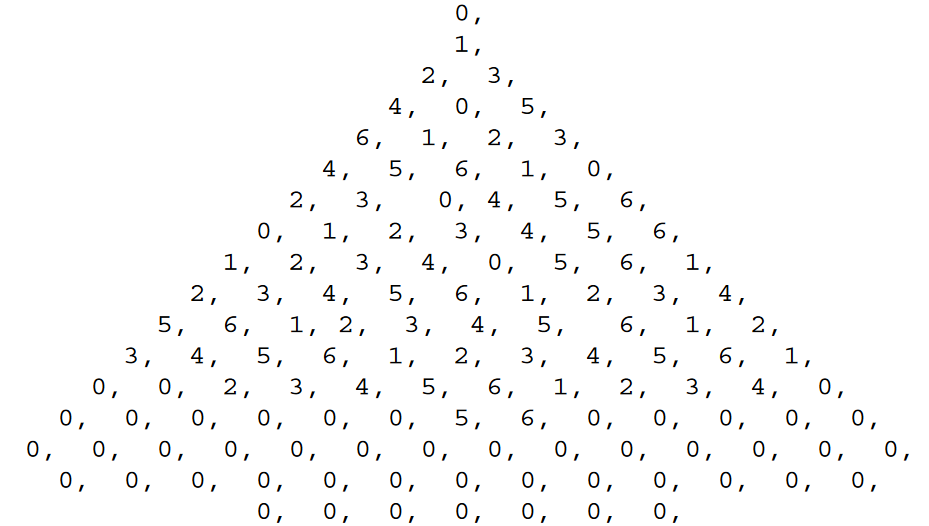
\includegraphics[width=0.6\linewidth]{cartogram.png}}
    \caption{Картограмма порядка выгрузки ТВС для программного средства RERPRORYV}
    \label{pic:cartogram}
    \end{figure}

Схема перегрузок подразумевает задание групп ТВС,  которые выгружаются по окончании очередной микрокампании (рис. \ref{pic:cartogram}). 
При этом выгружаются не все ТВС из активной зоны,  а только их часть,  через год  --  ещё одна часть,  через ещё год  --  ещё одна и т .д . 
Пользователь может задать,  какую часть активной зоны необходимо будет выгружать каждый год. 
Перестановок ТВС внутри активной зоны нет \cite{reproryv}.


\section{Выводы по главе}

В данной главе приведен обзор устройства ядерного реактора на примере реактора БН-350.
Рассмотрны основные конструкционные элементы, а также произведен разбор процесса перегрузки ядерного топлива.

Выполнен сравнительный анализ существущих программных средств, применяемых для планирования перегрузки: TRIGEX, САПФИР\_95, RC\_ВВЭР, REPRORYV.
Выявлено, что существующие программные комплексы способны проводить расчет либо только для стационарных схем перегрузки, либо по заданной вручную схеме.

Таким образом, необходимо разработать метод для оптимизации технологических процессов ядерных реакторов на примере процесса перегузки ядерного топлива.